\subsection{Eliminazione di una Rete Bayesiana}\label{EliminazioneRete}

Accanto alla selezione di una rete bayesiana già caricata (§\ref{SelezioneRete}) esiste anche l'operazione speculare di rimozione di una rete bayesiana memorizzata nel server.\\
Anche questa operazione consta di due passaggi, di cui il primo assolutamente analogo all'operazione precedente:
\begin{enumerate}
	\item \textbf{Passaggio 1:} L'utente seleziona, attraverso l'apposito menù a tendina visibile in Figura \ref{SelezioneReteImg} una delle reti bayesiane memorizzate nel server;
	\item \textbf{Passaggio 2:} L'utente conferma l'eliminazione della rete attraverso il pulsante \textbf{Elimina}.
\end{enumerate}

A seguito della corretta rimozione della rete bayesiana l'utente verrà avvisato del buon esito dell'operazione da un messaggio di notifica (Figura \ref{NotificaRimozioneRete}). La rete in questione, insieme alle relative impostazioni di collegamento, verrà rimossa sia dal pannello che dal server.

\begin{figure}[H]
	\begin{center}
		
\includegraphics[scale=0.6]{./images/NotificaRimozioneRete.png}
		 \caption{Notifica di Avvenuta Rimozione della Rete Bayesiana}	
		 \label{NotificaRimozioneRete}
	\end{center}
\end{figure}

\textbf{\textcolor{red}{ATTENZIONE}}: Nel caso in cui l'utente abbia scelto di eliminare una rete al momento sotto monitoraggio attivo l'operazione non va a buon fine e l'utente viene avvisato di tale risultato da un messaggio di errore (Figura \ref{ErroreDeleteNet}).

\begin{figure}[H]
	\begin{center}
		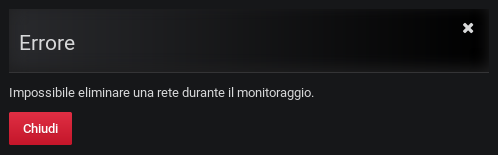
\includegraphics[scale=0.6]{./images/ErroreDeleteNet.png}
		 \caption{Messaggio di Errore Eliminazione di una Rete Bayesiana}	
		 \label{ErroreDeleteNet}
	\end{center}
\end{figure}
